\documentclass[12pt]{article}

\input preamble

\title{Principles of Parallel Architecture\\
Project Report 2}
\author{Xitong Liu \\
xliu@ece.udel.edu}

\begin{document}

\maketitle

\section{Introduction}
In this report, we will introduce the methods applied to optimize
the performance of Matrix Multiplication on parallel architecture.
Results showed that the performance has been improved a lot comparing
to the baseline approach proposed in the previous report.

\section{Baseline}
The setup of the baseline parallel is straightforward, as we divide
one matrix operand evenly into several parts, each part is distributed
to one thread. The approach is shown in Figure\ref{fig:matrix-divide}.

\begin{figure}[h!]
	\begin{center}
		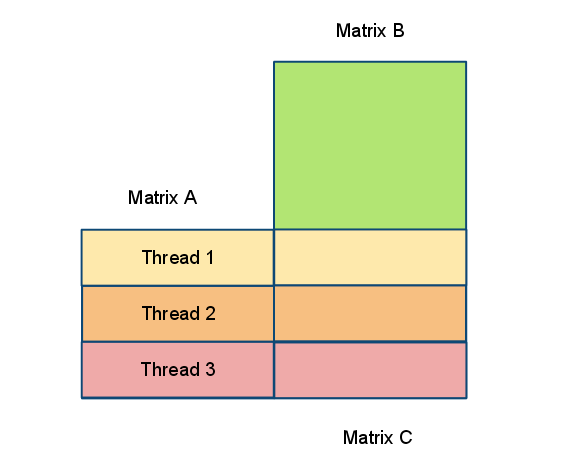
\includegraphics[width=0.5\textwidth]{matrix-divide.png}
		\caption{\label{fig:matrix-divide}Divide the matrix 
			evenly by the number of threads}
	\end{center}
\end{figure}

\section{Cache Line}
The 
\begin{verbatim}
DO I = 1, N 
  DO J = 1, N
	  C(J,I) = 0.0 
      DO K = 1, N
      C(J,I) = C(J,I) + A(J,K) * B(K,I) 
    ENDDO
  ENDDO
ENDDO
\end{verbatim}
\begin{figure}[h!]
	\begin{center}
		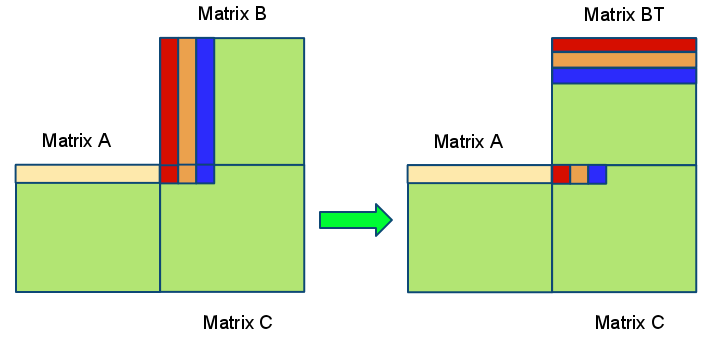
\includegraphics[width=0.7\textwidth]{cacheline.png}
		\caption{\label{fig:cacheline}Transpose the matrix to utilize
		the benefits from cache line}
	\end{center}
\end{figure}

\end{document}

\begin{comment}
\begin{figure}[h!]
	\begin{center}
		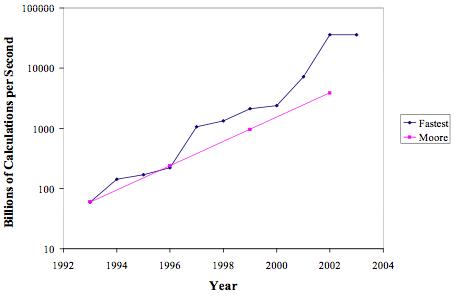
\includegraphics[width=0.7\textwidth, angle=0]{fatest.png}
		\caption{\label{fig:fatest}Fatest SuperComputer in the world}
	\end{center}
\end{figure}
\end{comment}